\section{Transport of spinless BECs in speckle potentials}\label{transport}

In chapter (\ref{chpt 5}), we study the transport of spinless BECs under speckle potentials. As Fig.~ (\ref{fig:single}) shows, a BEC with chemical potential $~300 {\rm Hz}$ travel through speckle potentials with average potential depth $~200 {\rm Hz}$ could be scattered by the speckle potential and decelerate. The deceleration of a BEC depends on its initial velocity and the cutoff $k_c$ in the speckle potential PSD. As Fig.~ \ref{fig:single}(d) shows, after evolving under the speckle potential for $16 {\rm mm}$, the BECs with small initial velocity has more significant deceleration. For BECs with large initial velocity, $k_0>k_c/2$, the deceleration is minimal during the $16 {\rm mm}$.

In experiment, we would like to see how BECs with different velocities decelerate. As discussed in chapter (\ref{speckle_chapter}), we can make speckle potentials that have the same PSD as our numerical simulation. And as discussed in Sec. ~(\ref{speckle_pulsing}), the average speckle potential depth can be measured. So an ideal experimental sequence is to have the BEC travel with constant velocity under well calibrated speckle potential, and the final velocity would be measured by using in-situ or TOF absorption images. To that end, the first challenge we are faced with is that how to make a BEC travel with a constant velocity for an extensive amount of time ($16 {\rm mm}$ in the simulation). We make BECs by doing evaporative cooling in a crossed dipole trap as discussed in Sec.~(\ref{dipole trap}), so our first choice is to make BECs travel in the crossed dipole trap. As Eq.~(\ref{dipole_poten}) suggests, dipole potential is proportional to the intensity of the dipole beam. 

In our case, we image atoms in z direction and measure the motion of atoms in x direction. The dipole potential in x direction is a combination of the dipole potential from z dipole beam and x dipole beam. The width of the dipole potential from x dipole beam is the Rayleigh length, which in our case is $~ 1.3{\rm mm}$. Based on our design, the velocity of atoms corresponds to the recoil $k$ vector $k_r$ is $3.3 {\rm \mu m/ms}$. We expect the atoms to move less than $50 {\rm \mu m}$ during the experiment, so the dipole potential from x dipole beam can be ignored.

In x direction, the dipole potential from the z dipole beam is
\begin{equation}
    V_{dip}(x) = -V_0\exp{-\frac{2x^2}{w^2}}.
\end{equation}
where $w$ is the width of the beam at the atoms. Expand the potential at $x=0$ to second order,
\begin{equation}
    V_{dip}(x) \approx -V_0 + \frac{2V_0}{w^2}x^2,
\end{equation}
has a quadratic form. Around the center of the trap, the dipole potential can be approximated by a harmonic potential with frequency $\sqrt{\frac{4V_0}{w^2}}$.

In the ideal case, the atoms would move at a constant velocity in the dipole trap, meaning the frequency $\sqrt{\frac{4V_0}{w^2}}$ is zero and the z dipole beam is completely turned off. More realistically, if the velocity of the atoms change by less than 5\% at the center of the trap in $15 {\rm ms}$, the period of the harmonic oscillation needs to be more than $300 {\rm ms}$. So the trapping frequency is around $3 {\rm Hz}$. 

The x dipole beam and the z dipole beam in our experiment are the first order and zeroth order beams from an AOM, the total power of the two beams are conserved. We optimized the ratio of power of the two beams to maximize the phase space density of the BECs after the dipole evaporation stage. In the optimized case, the measured trapping frequency in x direction is $21 {\rm Hz}$. In order to decrease the x trapping frequency, we need to allocate more power in the x dipole beam and less in the z dipole beam. But in the process of decreasing the x trapping frequency, a few problems occurred. 

Fig. \ref{fig:lower trapping freq} shows the BEC with x trapping frequency of $21 {\rm Hz}$ compared with the BEC with x trapping frequency of $5.8 {\rm Hz}$. Compared with the BEC in Fig. \ref{fig:lower trapping freq}(a), the BEC in Fig. \ref{fig:lower trapping freq}(b) is stretched in the x direction due to small trapping frequency. The signal is much weaker and the extension in x direction makes it hard to accurately detect the center of the BEC and the center-of-mass motion.

\begin{figure*}
    \centering
    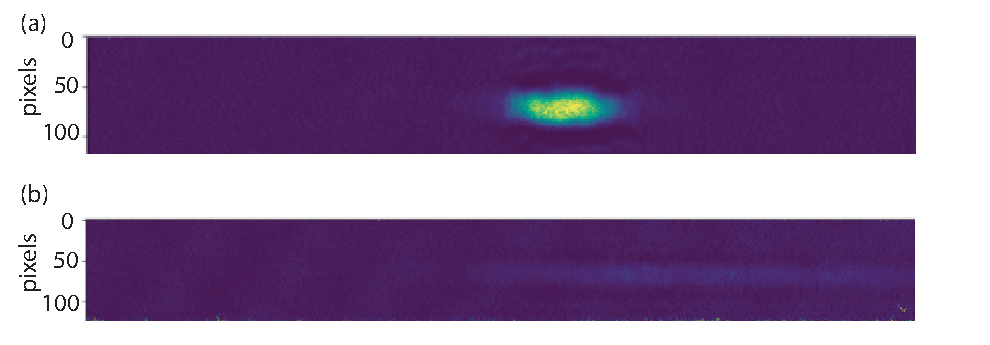
\includegraphics{Chapter6_secs/decrease_trap_freq.pdf}
    \caption{$In~situ$ absorption images of BECs with different dipole parameters. (a) A BEC with x trapping frequency of $21 {\rm Hz}$. (b) A BEC with x trapping frequency of $5.8 {\rm Hz}$}
    \label{fig:lower trapping freq}
\end{figure*}

Alternatively, we can keep the current dipole trap configuration and decrease the time that BECs travel under speckle potentials. We hope to find the duration of the speckle potential pulses that is as short as possible but its deceleration effect of BECs is significant. In Fig. \ref{fig:deceleration_in_dip_osc}, the blue dots show the oscillation of a BEC in x direction in a dipole trap with x trapping frequency $21 {\rm Hz}$. The center of the atoms is measured from $in situ$ images of atoms. At the center of the dipole trap, the atoms are at the maximum velocity $v_0$, $mv_0/\hbar = 1.8k_r$. The first time the atoms reaches maximum velocity is at $21 {\rm ms}$. We make the atoms do the same dipole oscillation as the blue dots show, at $21 {\rm ms}$, we turn on the speckle potential and hold for $1 {\rm ms}$. After $1 {\rm ms}$, the speckle potential is turned off and we track the center-of-mass motion of the atoms in x direction in the dipole trap. The center-of-mass motion of atoms after the speckle pulse is shown as the orange dots in Fig. \ref{fig:deceleration_in_dip_osc}. 

\begin{figure*}
    \centering
    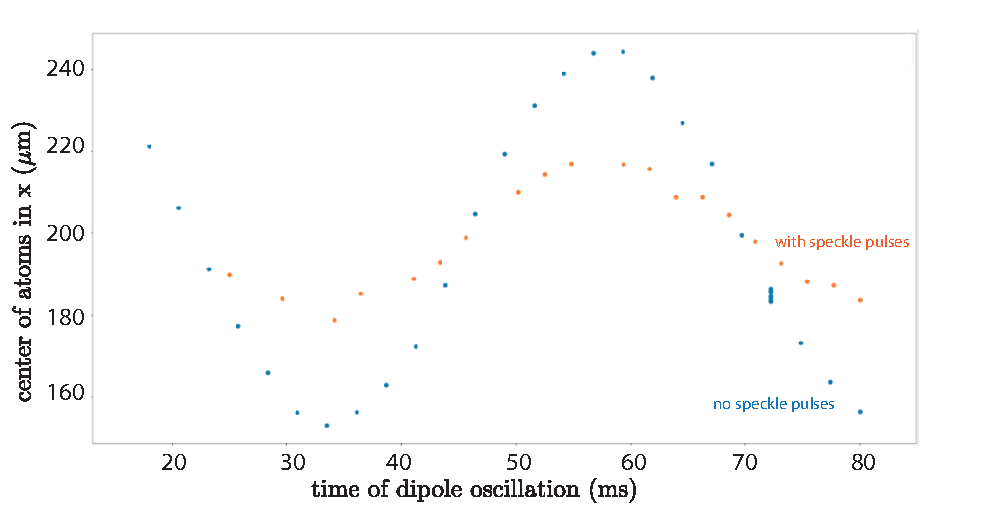
\includegraphics{Chapter6_secs/deceleration_in_dip_osc.pdf}
    \caption{Center of mass motion in x direction of atoms during dipole oscillation. The blue dots show a full cycle of dipole oscillation without pulses of speckle potential. The orange dots show the dipole oscillation of atoms with the same initial velocity as the blue dots show, but with a $1 {\rm ms}$ speckle pulse at $21 {\rm ms}$. The average speckle potential depth is $\approx 640 {\rm Hz}$.}
    \label{fig:deceleration_in_dip_osc}
\end{figure*}

The amplitude of the oscillation shown by the orange dots is smaller than the amplitude shown by the blue dots. We fit a sinusoidal function to both and infer the velocities of the atoms at $t=21 {\rm ms}$. Without the pulse of speckle potential at $t=21 {\rm ms}$, the velocity of the atoms is $v_0$, $mv_0/\hbar = 1.8k_r$. With the pulse, the velocity of the atoms is $v_f$, $mv_f/\hbar = 0.7k_r$. This measurement demonstrated that a speckle potential with average potential depth of $\approx 640 {\rm Hz}$, can have significant deceleration effect on atoms within $1 {\rm ms}$. This allows us to measure the deceleration of atoms evolving in speckle potentials in our optimized dipole trap, without having to reduce the x trapping frequency.

Using this method, we measured the deceleration of atoms at different velocity $v_0$ after pulses of speckle potential with average potential depth of $\approx 500 {\rm Hz}$ for $1 {\rm ms}$. Fig.~\ref{fig:spinless transport} shows the experimental measurements compared with the numerical simulation results. The red circles in Fig.~\ref{fig:spinless transport} show the experimental results. In the numerical simulations, we make atoms with different initial velocity evolve under speckle potentials with different potential depth for $1 {\rm ms}$ and measure the final velocity. The initial velocities range from $0.2\frac{\hbar k_r}{m}$ to $2.2\frac{\hbar k_r}{m}$. The blue curve and the yellow curve in Fig.~\ref{fig:spinless transport} correspond to speckle potential depth of $500 {\rm Hz}$ and $800 {\rm Hz}$, respectively. In experiment, the average speckle potential depth is inferred from Fig.~\ref{fig:avg_speckle_poten}. As discussed in Sec.~\ref{long_pulse}, we use the stationary width of momentum distribution after long-term speckle pulses to measure the average speckle potential. Here the deceleartion measurement is done with PD reading $1.0 {\rm V}$, which corresponds to an average speckle potential of $\approx 500 {\rm Hz}$. The measured final velocity $v_f = \frac{\hbar k_r}{m}$ is lower than the final velocity in the simulation with average speckle potential of $500 {\rm Hz}$ and close to the simulation with average speckle potential of $800 {\rm Hz}$. The uncertainty in the measurement of the stationary width of momentum distribution after long-term pulses of speckle potential can be a cause that leads to the gap.

\begin{figure*}
    \centering
    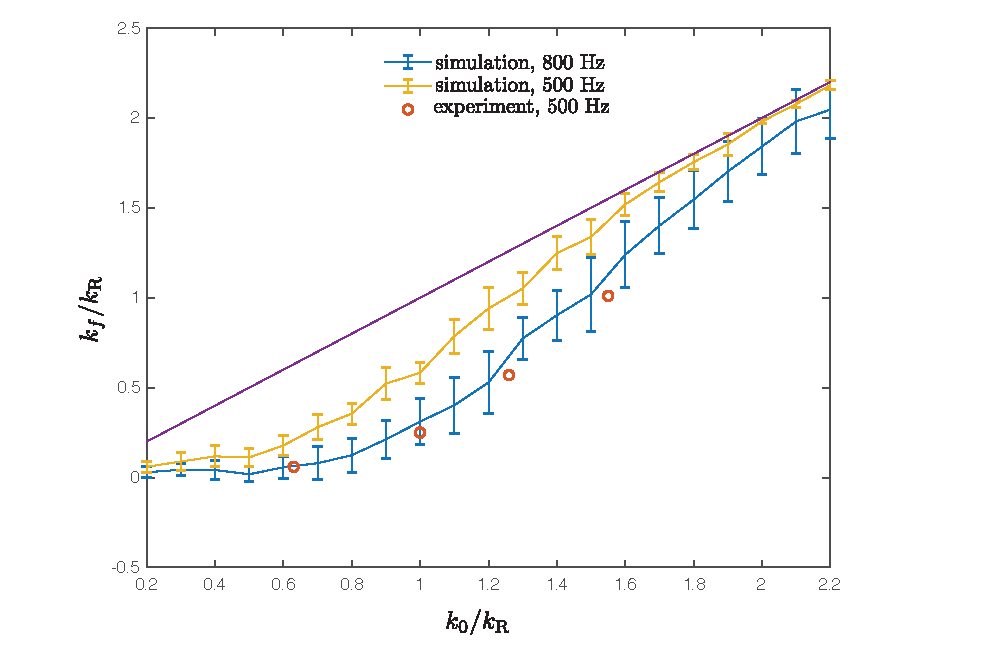
\includegraphics{Chapter6_secs/spinless_transport.pdf}
    \caption{Deceleration of atoms after a $1 {\rm ms}$ pulse of speckle potentials. The red circles are the results of measurement in the experiment. The average speckle potential depth inferred from the photo diode reading is $\approx 500 {\rm Hz}$. The blue curve and the yellow curve are the results of numerical simulation. The blue curve is final velocity vs initial velocity after evolving under speckle potential with average potential depth of $800 {\rm Hz}$, and the yellow curve is for speckle potential with average potential depth of $500 {\rm Hz}$. Both the blue curve and the yellow curve are averaged over 20 speckle realizations and the error bars show the standard deviation. The purple line is $k_f=f_0$. }
    \label{fig:spinless transport}
\end{figure*}